\documentclass{report}

\usepackage{amsmath}
\usepackage{geometry}
\usepackage{amsfonts}
\usepackage[english]{babel}
\usepackage{amssymb}
\usepackage{graphicx}
\usepackage{float}
\usepackage{hyperref}
\usepackage{multirow}
\usepackage{pdflscape}
\usepackage{caption}
\usepackage{pdflscape}
\usepackage{outlines}
\usepackage{subcaption}
\usepackage{enumerate}
\usepackage[latin1]{inputenc}

\usepackage{tabularx, booktabs}
\usepackage{longtable}

\usepackage{standalone}

\usepackage[autostyle, english = american]{csquotes}
\MakeOuterQuote{"}

\usepackage{comment}

\newcommand{\tabnotes}[2]{\bottomrule \multicolumn{#1}{@{}p{0.95\linewidth}@{}}{\footnotesize #2 }\end{tabular}\end{table}}

\title{PCR and Measurement Error}
\author{Isaac Liu}
\date{\today}

\setlength{\parindent}{0pt}
\setlength{\parskip}{0.5em}

\hypersetup{
    colorlinks=true,
    linkcolor=blue,
    filecolor=magenta,      
    urlcolor=cyan,
}

\begin{document}

	\maketitle

	\newpage \clearpage

    \section*{Application: Government Share of Healthcare Spending and Life Expectancy}

	% Add \ref to the following table?
	In the left column in the table below I first regress the life expectancy at birth for all individuals in a given country and year on a measure of government spending as a share of total health expenditure. In the middle column I include the economic controls/covariates of GDP per capita (PPP), GNI per capita (PPP), Survey Mean Income/Consumption Per Capita, ILO GDP per person employed, and Net Foreign Assets Per Capita, all from the World Bank. In the rightmost column I instead use the first principal component combining these covariates.
	
	I standardize all variables by subtracting the mean and dividing by the standard deviation, linearly interpolate data between known observations, and remove country-years with missing values for any of the economic indicators.

    \begin{table}[!htbp] \centering
\begin{tabular}{@{\extracolsep{5pt}}lccccc}
\\[-1.8ex]\hline
\hline \\[-1.8ex]
& \multicolumn{5}{c}{\textit{Life Expectancy at Birth (Years)}} \
\cr \cline{5-6}
\\[-1.8ex] & (1) & (2) & (3) & (4) & (5) \\
\hline \\[-1.8ex]
 Govt. Share of Health Exp. & 0.549$^{***}$ & 0.271$^{***}$ & 0.022$^{***}$ & 0.289$^{***}$ & 0.024$^{***}$ \\
  & (0.019) & (0.018) & (0.007) & (0.018) & (0.007) \\
 Covariates & None & Econ Indicators & Econ Indicators & PCs & PCs \\
 Fixed Effects & No & No & Yes & No & Yes \\
\hline \\[-1.8ex]
 Observations & 1,994 & 1,994 & 1,994 & 1,994 & 1,994 \\
 $R^2$ & 0.302 & 0.546 & 0.987 & 0.510 & 0.987 \\
 Adjusted $R^2$ & 0.301 & 0.543 & 0.985 & 0.510 & 0.985 \\
 Residual Std. Error & 0.836 & 0.676 & 0.120 & 0.700 & 0.121  \\
 F Statistic & 859.952$^{***}$  & 198.486$^{***}$  & 1460.518$^{***}$  & 1037.286$^{***}$  & 4740.757$^{***}$  \\
\hline
\hline \\[-1.8ex]
\textit{Note:} & \multicolumn{5}{r}{$^{*}$p$<$0.1; $^{**}$p$<$0.05; $^{***}$p$<$0.01} \\
 & \multicolumn{5}{r}\textit{All variables are standardized.} \\
\end{tabular}
\end{table}

	% Though the coefficients are not readily interpretable, they do differ from each other

	% ADD TEST to show coefficients differ? I think this also would not be easy to interpret since the independent variables are different...

	% In both cases, they are significant.
	
	% Notably, we demonstrate a higher $R^2$ using the principal component model.

	\newpage \clearpage

    \section*{With Ginis instead of econ controls}

	\begin{table}[!htbp] \centering
\begin{tabular}{@{\extracolsep{5pt}}lccccc}
\\[-1.8ex]\hline
\hline \\[-1.8ex]
& \multicolumn{5}{c}{\textit{Life Expectancy at Birth (Years)}} \
\cr \
\\[-1.8ex] & (1) & (2) & (3) & (4) & (5) \\
\hline \\[-1.8ex]
 Govt. Share of Health Exp. & 0.697$^{***}$ & 0.652$^{***}$ & 0.028$^{}$ & 0.692$^{***}$ & 0.026$^{}$ \\
  & (0.034) & (0.040) & (0.024) & (0.037) & (0.023) \\
 Covariates & None & Ginis & Ginis & PCs & PCs \\
 Fixed Effects & No & No & Yes & No & Yes \\
\hline \\[-1.8ex]
 Observations & 322 & 322 & 322 & 322 & 322 \\
 $R^2$ & 0.566 & 0.596 & 0.999 & 0.566 & 0.999 \\
 Adjusted $R^2$ & 0.565 & 0.583 & 0.998 & 0.564 & 0.998 \\
 Residual Std. Error & 0.596 & 0.583 & 0.040 & 0.597 & 0.040  \\
 F Statistic & 417.382$^{***}$  & 45.905$^{***}$  & 1421.063$^{***}$  & 208.238$^{***}$  & 5197.564$^{***}$  \\
\hline
\hline \\[-1.8ex]
\textit{Note:} & \multicolumn{5}{r}{$^{*}$p$<$0.1; $^{**}$p$<$0.05; $^{***}$p$<$0.01} \\
 & \multicolumn{5}{r}\textit{All variables are standardized.} \\
\end{tabular}
\end{table}

	\newpage \clearpage

    \section*{Health share of gdp}

	\begin{table}[!htbp] \centering
\begin{tabular}{@{\extracolsep{5pt}}lccccc}
\\[-1.8ex]\hline
\hline \\[-1.8ex]
& \multicolumn{5}{c}{\textit{Life Expectancy at Birth (Years)}} \
\cr \cline{5-6}
\\[-1.8ex] & (1) & (2) & (3) & (4) & (5) \\
\hline \\[-1.8ex]
 GDP Share of Health Exp. & 0.258$^{***}$ & 0.184$^{***}$ & -0.024$^{}$ & 0.144$^{***}$ & -0.020$^{}$ \\
  & (0.023) & (0.019) & (0.031) & (0.017) & (0.030) \\
 Covariates & None & Econ Indicators & Econ Indicators & PCs & PCs \\
 Fixed Effects & No & No & Yes & No & Yes \\
\hline \\[-1.8ex]
 Observations & 1,799 & 1,799 & 1,799 & 1,799 & 1,799 \\
 $R^2$ & 0.067 & 0.553 & 0.987 & 0.467 & 0.987 \\
 Adjusted $R^2$ & 0.066 & 0.549 & 0.985 & 0.467 & 0.985 \\
 Residual Std. Error & 0.967 & 0.672 & 0.122 & 0.730 & 0.123  \\
 F Statistic & 128.396$^{***}$  & 146.946$^{***}$  & 772.041$^{***}$  & 787.819$^{***}$  & 384.737$^{***}$  \\
\hline
\hline \\[-1.8ex]
\textit{Note:} & \multicolumn{5}{r}{$^{*}$p$<$0.1; $^{**}$p$<$0.05; $^{***}$p$<$0.01} \\
 & \multicolumn{5}{r}\textit{All variables are standardized.} \\
\end{tabular}
\end{table}

    \clearpage \newpage

    \appendix

    \section*{Appendix}

	\begin{figure}[h!]
		\centering
		\caption{Correlations Between Covariates and Life Expectancy}
		\label{LE_Health_Econ_Correlations}	
		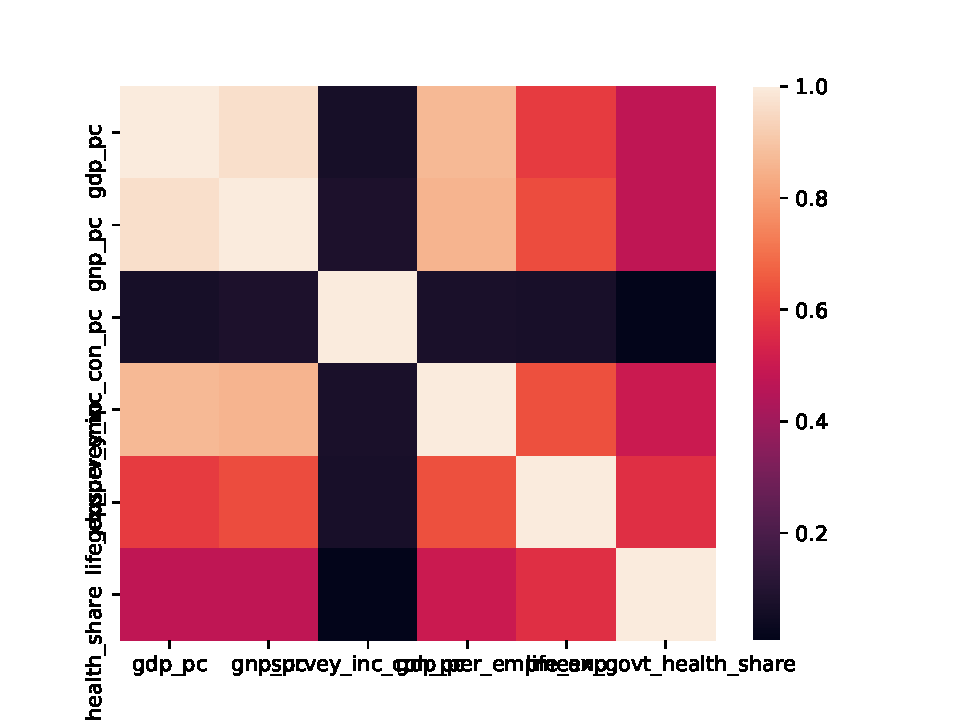
\includegraphics[width=\linewidth,keepaspectratio=true]{../Output/Figures/LE_Health_Econ_Correlations.pdf}
	\end{figure}

	\begin{figure}[h!]
		\centering
		\caption{Economic Measures PCA Loadings}
		\label{Econ_Loadings}	
		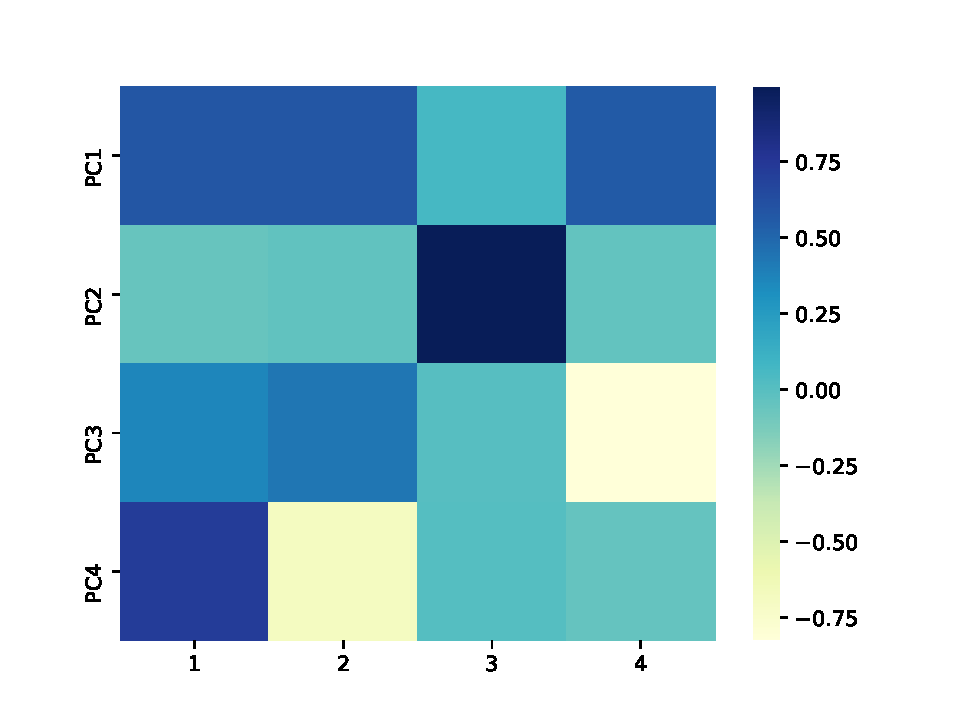
\includegraphics[width=\linewidth,keepaspectratio=true]{../Output/Figures/Econ_Indicator_Loadings.pdf}
	\end{figure}

	\begin{figure}[h!]
		\centering
		\caption{Economic Measures PCA Share of Variance Explained}
		\label{Econ_Share_Explained}	
		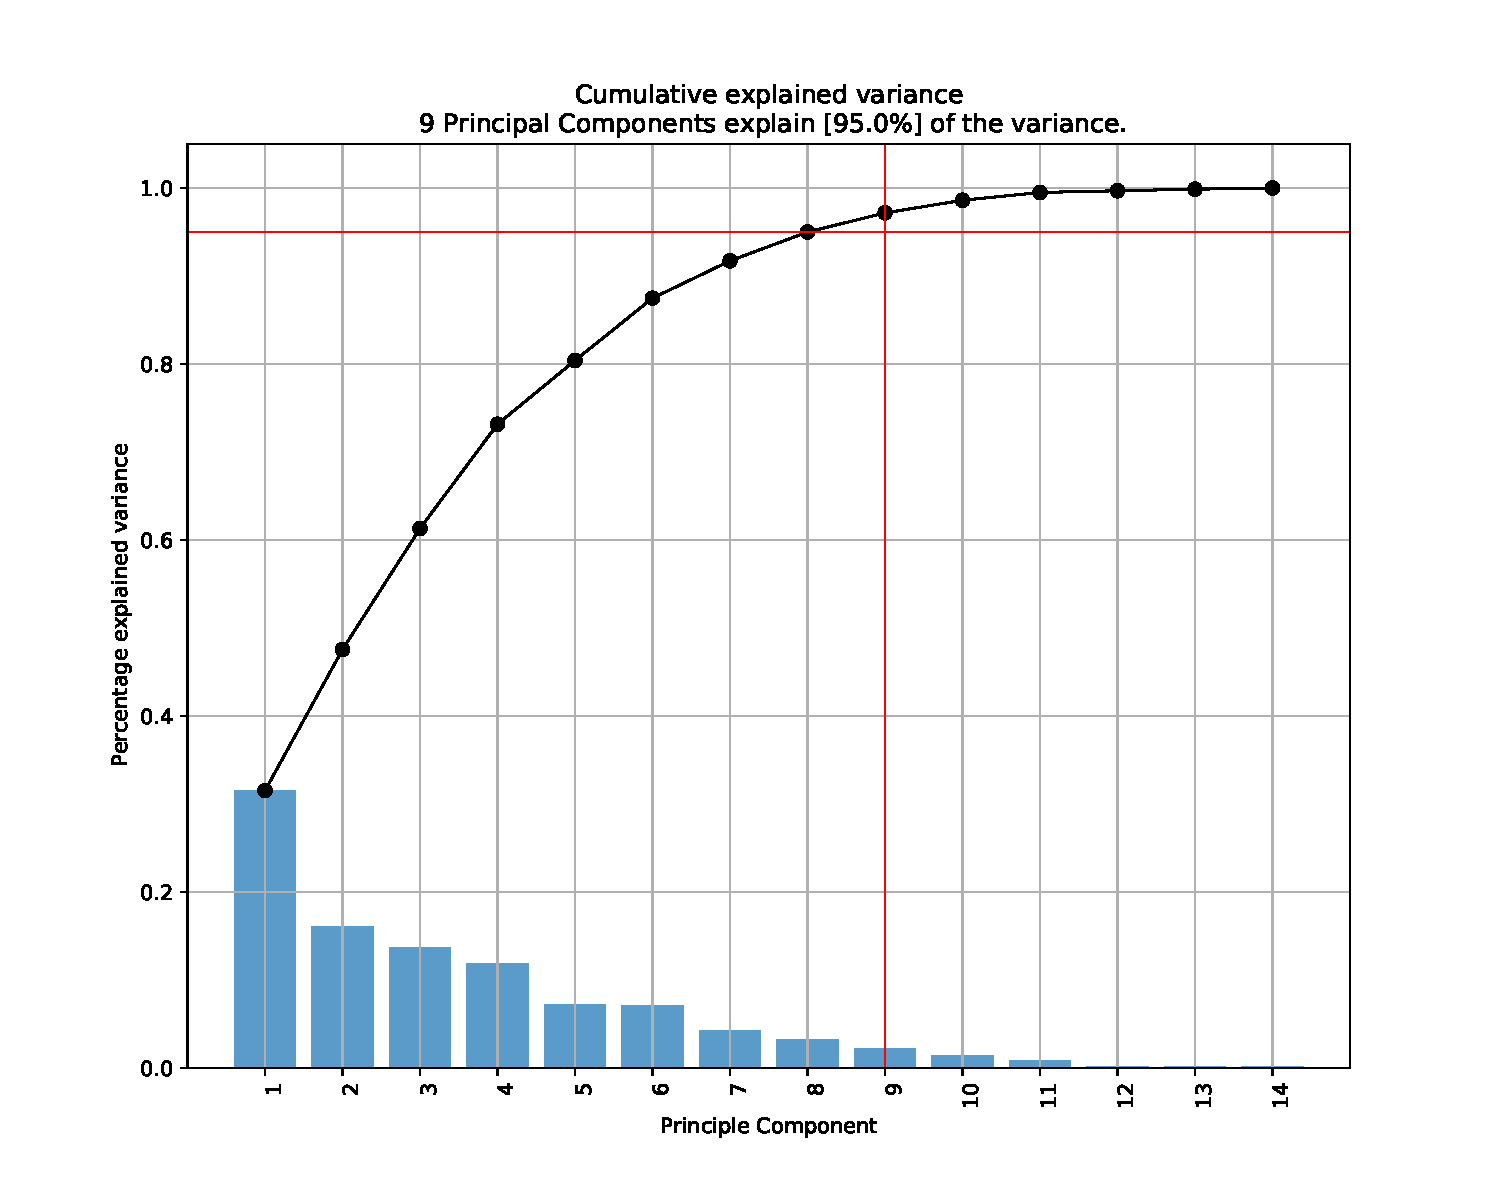
\includegraphics[width=\linewidth,keepaspectratio=true]{../Output/Figures/Econ_Indicator_Share_Explained.pdf}
	\end{figure}

\end{document}